\subsection{Co-expressed networks} \label{s:lit:co_net}

\vspace{3mm}
% \noindent\rule{17cm}{0.2pt}
\fbox {
    \parbox{\linewidth}{
      \begin{itemize}
        \item Weighted Gene Correlation Network Analysis (WGCNA)
        \item Parsimonious Gene Correlation Network Analysis (PGCNA)
      \end{itemize}
    }
}
\vspace{3mm}

There are two methods reviewed in this section: \acrlong{wgcna} (WGCNA - \citet{Langfelder2008-sn}) and Parsimonious Gene Correlation Network Analysis (PGCNA - \citet{Care2019-ij}). The latter was developed with the goal of combining multiple datasets to stratify a disease, whereas the former was primarily focused on analysing co-expressed networks and it is the first method to formalise the co-expressed network approach. Despite their distinct goals, the two approaches share common steps in the network construction process but have different caveats:

\begin{enumerate}
    \item \textbf{Network Construction:} The network is constructed based on the correlation matrix. In this step, WGCNA modifies the correlation values to fall between 0 and 1, whereas PGCNA maintains the original correlation values without any alterations.
    
    \item \textbf{Edge Reduction:} The objective of this step is to distinguish significant signals from noise, thereby simplifying the network analysis. PGCNA adopts an aggressive strategy for edge reduction, while WGCNA only considers correlations that exceed a specified threshold.
    
    \item \textbf{Reconstruction from Reduced Matrix:} Following the reduction of edges, the network is reconstructed from the reduced matrix to include only significant correlations.
    
    \item \textbf{Community Detection:} In the final step, communities within the network are identified. WGCNA employs hierarchical clustering methods, while PGCNA uses community detection algorithms such as Louvain \citep{Blondel2008-ik} or Leiden \citep{Traag2019-ne}.
\end{enumerate}

\gls{PGCNA} involves additional computational steps that extract the most relevant genes in each community, then find their representation in the gene expression dataset, values which are subsequently clustered to define the subtypes. These steps are discussed in more detail in the PGCNA \cref{s:lit:pgcna}.


 % WGCNA
\paragraph*{WGCNA} \label{s:lit:WGCNA}

One of the most popular \acrfull{gcna} is the WGCNA by \citet{Langfelder2008-sn}. This paper is an accumulation of different works from Dr Steve Horvath lab which offers a clear and concise methodology to build and analyse a GCN, and more importantly everything is packed in an R package which can then be used by researchers. Being a referential work in the field, it follows the steps described above on creating, processing and analysing the graph.

Compared to PGCNA (see \cref{s:lit:pgcna}) where correlation values are unaltered, in WGCNA the values are scaled from 0-1 at the cost of losing information resolution but of improving the graph processing. To reduce the number of edges, the authors sets a threshold to the correlation values (default to $0.02$) and for community detection they apply topological overlap which has been described in \cite{Zhang2005-xq} and applied in \citep{Yip2007-mr, Li2007-vz, Ravasz2002-au}. The discovered modules are then clustered using hierarchical clustering.

\gls{WGCNA} has been successfully used to a large number of applications from analysing the transcriptome for normal/failing Murine Hearts \citep{Lee2011-wm} or to find the regulatory genes/pathways related with obesity in pigs \citep{Kogelman2014-ea}, and to human cancer \citep{Yang2014-wv, Clarke2013-wd, Care2019-ij}. The wide range shows the versatility of the model and the power of co-expressed networks. However, as it will be shown in the next section and in the work of \citet{Care2019-ij}, PGCNA yields more biologically significant communities compared to WGCNA (measured by enrichment score and adjusted to community size).

% PGCNA
\paragraph*{PGCNA} \label{s:lit:pgcna}

\acrlong{pgcna} \citep{Care2019-ij}, is a more recent approach developed with the goal to stratify a disease based on gene expression and help researchers visualise using the genomic data exploration. The authors' goals closely align with the ones set for this project with a few differences. The work done in this thesis aims to built a method which will enable the integration of multiple data types whereas the PGCNA combines multiple datasets of the gene expression. 

The authors compare their work with WGCNA and draw inspiration from other techniques that re-construct the regulatory network of tissues from microarrays and use Mutual Information (MI - \citet{Margolin2006-mc,Zhang2013-fs}) to calculate gene pair-wise relationship. Compared to correlation scores MI is a more general method to describe the dependence between two variables by using information theory concepts, but it is also harder to interpret.


% Alternatives to co-expressed networks - partial-coor
\paragraph*{Partial-correlation} \label{s:lit:partial-corr}

Both PGCNA and WGNNA use the Spearman or Pearson correlation and an alternative metric is the partial-correlation which removes the influences of other variables to the correlation of the studied pair of variables, thus giving a purer correlation metric. This approach has been applied by \citet{De_la_Fuente2004-ts} to a yeast microarray gene expression.  For partial-correlation to work, the dataset has to be symmetric, the number of samples and features equal. This is not the case for genomic data where there are more features than samples. One finding from simulated data is that there is no added value for computing more than the second order partial correlation\footnote{Second-order refers to how many variables are controlled so as not to affect the relationship between the studied pair of variables. For example, calculating the second-order partial correlation for $x$ and $y$ means removing the effect of variable $a$ and $b$}. This is relevant because each order of the partial correlation introduces an added computational cost. \citet{De_la_Fuente2004-ts} generated some biological leads but were never assessed in term of thei successf. Nevertheless, partial-correlation remains an alternative to other popular metrics that can be further explored.

The partial-correlation is also known as the inverse of the covariate matrix or precision metrics and there has been work to make it more efficient \citep{Ghanbari2019-tq}. However, this is not a widely used metric in building the biological networks arguably due to the small number of samples over the features and the more computationally taxing process to the alternatives.

\subsection{Network pipeline}

\vspace{3mm}
% \noindent\rule{17cm}{0.2pt}
\fbox {
    \parbox{\linewidth}{
      \begin{itemize}
        \item Creating the network
        \item Edge reduction
        \item Community detection
        \item Bridging the gap between the genes and samples
      \end{itemize}
    }
}
\vspace{3mm}

\paragraph*{Building the network} 

As the previous methods have shown, the PGCNA supports the integration of multiple gene expression datasets by taking the median expression of a gene across the data. It has also been released in a GitHub package\footnote{\href{https://github.com/medmaca/PGCNA}{PGCNA Github repository}} and is relatively easy to use and adapt to one's needs. PGCNA was also successfully applied to the Breast and Glioblastoma cohorts from TCGA and it supports multiple datasets by using the median gene expression.

\paragraph*{Edge reduction}

One important finding in the work of \citet{Care2019-ij} is that a simple and aggressive edge pruning strategy performed better than other strategies. These were iPCC (iterative Pearson’s correlation coefficient), PowerST and Sigmoid, the last two being part of the WGCNA pipeline.

The authors explored keeping edges from 3-10 and all of them, and found that less than three yielded isolated communities (or disconnected). Also, by increasing the numbers yielded a large number of communities find and a decrease in the SCES metric (modularity score too). An inverse relationship between the minimum number of edges allowed for a gene and the community detection performance was also observed in this project in \cref{s:N_I:sel_pruning}.

\paragraph*{Community detection}

To detect the network sub-structures after the correlation matrix was reduced, the \citet{Care2019-ij} explored three different classes of algorithms: K-means, hierarchical clustering and community detection (Louivan - \cite{Blondel2008-ik} or FastUnfold Leiden - \cite{Traag2019-ne}\footnote{Leiden algorithm is an improvement to the Louivan which was released after PGCNA was published, but in the Github package, the Leiden is used as it outperforms Louivan.}). Leiden outperformed the other two algorithms, with Louivan applied to a network constructed with 3 edges per gene having the highest SCES. What is essential in this comparison is that the traditional clustering methods, K-means and hierarchical clustering, are outperformed by the network approach.

\paragraph*{Bridging the gap between genes and sample}

The end goal of PGCNA is to use the network representation to inform disease subtyping. There is therefore a need to bridge the gap between the gene representation and samples. This is done by using the module connection values (ModCon) which selects the top 25 most relevant genes from each community regardless of its size. The \gls{MEV} (MEV) takes the 25 genes and computes the enrichment in the dataset which are then used for subtyping. Both ModCon and MEV scores are used and adapted to the project aims and covered in more details in \cref{s:N_I:methods_modcon,s:N_I:mev}.

\paragraph*{Measuring success} 

To asses the performance of PGCNA over other techniques, \citet{Care2019-ij} proposed the scaled cluster enrichment score (SCES). The metric is computed for each module (i.e. a set of gene grouped together - regardless of the method, network or cluster analysis) taking into account the enrichment scores (obtained from gene ontology) and it selects the 15 most significant\footnote{Only the enriched pathways that have False-Discovery Rate (FDR) $<0.05$ and contain genes $\geq5$ between $\leq1000$}. Then, using z-scores, the specific enrichment is determined for each module. It is worth noting that the score is adjusted by the number of genes in a module. Therefore, SCES is a metric that rewards the modules with unique enrichment signals and that are not large or ‘rewarding purity' \citep{Care2019-ij}.

It is worth mentioning that gene ontology results are highly dependent on the list of genes given without receiving other necessary information such as fold change, which is used for \acrlong{gsea}. Moreover, the interval of genes contained is quite large, being rather permissive with the number of accepted enrichment.

Despite the limitations of gene ontology, SCES is a metric to asses the significance of the biology of each module which usually more than there is available for computational models.


\paragraph*{Remarks on PGCNA}

Overall, PGCNA represents a pipeline for disease subtyping which introduces several key methods to the field. It shows that network and community detection yields the best results, a simple edge pruning performs better than the other techniques and introduces methods to bridge the gap between the gene representation and the samples.

While PGCNA solves many of the challenges that this project has faced there are still others left untouched. How can other data types be integrated into the network approach? (\cref{s:N_I,s:N_II}) Would selective edge pruning offer a better representation of the data? (\cref{s:N_I:sel_pruning}) Thus, the work in this project takes inspiration from PGCNA, adapts it and it develops own methods to integrate multiple data types.

% Bayesian networks
\subsection{Bayesian approaches} \label{s:lit:bayesian}

An alternative to co-expressed network is provided by the work of \citet{Nakazawa2021-yq} which uses Bayesian methods, rather than the correlation metric, to construct the network of the cancer. The computationally expensive algorithm, initially introduced by \citet{Imoto2001-uc} was used by \citet{Tamada2011-ok} for implementation. Once the cancer’s network is built, the authors adapted the work of \citet{Tanaka2020-mw} to find patient specific subnetworks. Lastly, the patient-specific subnetworks are then clustered using the hierarchical clustering by their similarity and differences.

The work is applied to the stomach cancer from TCGA and it is compared to the subtypes from iCluster \citep{Shen2009-ew} (covered in \cref{s:lit:iCluster}) as a representative of the multi-omics approaches. iCluster was applied to the stomach TCGA cohort using somatic mutation, mRNA expression, miRNA expression, promoter methylation, somatic copy number alteration and protein expression. The authors \citet{Nakazawa2021-yq} argue that adding multi-omics introduces noise and pollutes the subtype discovery. The evidence presented is the lack of significance in survival rate in the TCGA paper which found four groups \citep{Cancer_Genome_Atlas_Research_Network2014-xp}. Using their method and only gene expression, they have found three subtypes that exhibited significant survival rates. The authors compared the method with iNMF \citep{Yang2016-dm}, another multi-omics clustering model that showed similar results with iCluster.

While \cite{Nakazawa2021-yq} performed Kaplan-Meier survival and gene ontology analysis, the authors do not delve deeply into the biological analysis and interpretation. One of their concluding points is that using multi-omics may introduce additional noise into subtyping. Based on the experiments conducted in this project, there was no evidence that mutations or Transcription Factors amplified the noise\footnote{Noise refers to irrelevant information that distracts from the true signal.} from gene expression. On the contrary, \cref{s:N_I:sel_pruning} demonstrates that prioritising TF through selective edge pruning identifies a subset of TF with known biological roles in bladder cancer and healthy datasets, and \cref{s:N_II:high_conn} shows that integrating mutation burden reveals another subset of genes with biological function in MIBC.


In summary, the research from \citet{Nakazawa2021-yq} represents a comparable Bayesian alternative to the work of \citet{Care2019-ij}, and the one developed in this project. While the aims are similar to the ones in this PhD, the work done here differentiates itself by the gene expression between both non-cancerous and cancerous data, transcription factors, and the mutations.


\subsection{Integrative methods} \label{s:lit:net_data_int}

\vspace{3mm}
% \noindent\rule{17cm}{0.2pt}
\fbox {
    \parbox{\linewidth}{
      \begin{itemize}
        \item Network propagation
        \item Work from \citet{Hofree2013-ld}
        \item Multi-layer
      \end{itemize}
    }
}
\vspace{3mm}


\paragraph*{Network propagation} \label{s:lit:net_prop}

An interesting approach to integrate multiple data types into a network is introduced by  \citet{Hofree2013-ld}. The authors created a network from public data on gene interaction networks \citep{Szklarczyk2019-pu, Cerami2011-ql, Lee2011-xj} to which they applied a projection method developed by \citet{Vanunu2010-el} to diffuse the somatic information into a gene interaction network. The resultant network is projected to a latent space using netNMF method \citep{Cai2008-fv} which represents the space combining the mutations and the gene expression. At the end hierarchical clustering is applied.

\citet{Hofree2013-ld} have applied the technique to ovarian, uterine and lung cancers cohorts from TCGA. They have explored the effects on the subtypes of these cancers, looked at the impact of synonymous and nonsynonymous mutations, and analysed the impact for each of the cancers. In addition, they replaced the somatic mutations with other data types from TCGA\footnote{CNV, methylation, mRNA expression, microRNA and protein profiles}. From this the authors observed that the type of data included depends on the disease type.

The pipeline introduced by \citet{Hofree2013-ld} is available to use at\footnote{The Python implementation is available on GitHub but it is not actively maintained \url{https://github.com/idekerlab/pyNBS}} and provides the opportunity to integrate multiple data types into a network. From the applications to the ovarian, uterine and lung cancers, the authors found potentially interesting biology such as the role of \textit{FGF} pathway in ovarian tumour. Another strength of the method is that it can be easy to interpret as seen in \cref{fig:lit:hofree} (Fig 5 from their paper).

The method from \citet{He2017-dj} uses a network propagation method to integrate somatic mutations in the network introduced in \citet{Vanunu2010-el} and then further developed by \citet{Hofree2013-ld}. The difference brought by \citet{He2017-dj} is that it creates an unweighted graph based on the Spearman correlation of the gene expression whereas \citet{Hofree2013-ld} applies the somatic mutations to gene interaction networks. Thus the latter does not use disease and patient specific information to derive the subtypes. The method of \citet{He2017-dj} outperforms the previous one developed by \citet{Hofree2013-ld}, but the methods are not as clearly presented and the software is not available for testing.

\begin{figure}[!b]
    \centering
    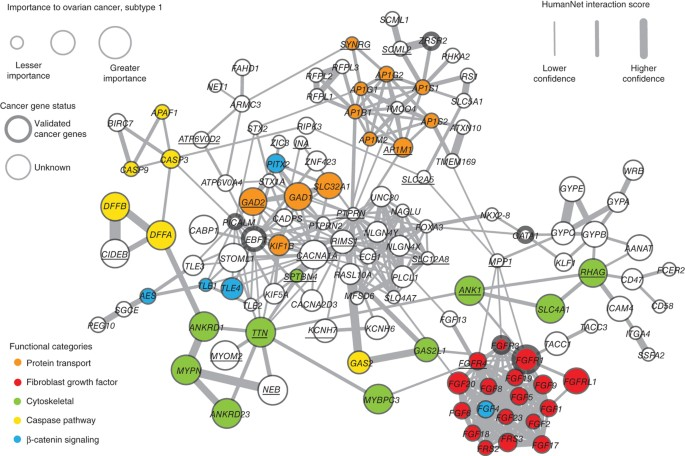
\includegraphics[width=1.0\textwidth,keepaspectratio]{Sections/Lit_review/Resources/hofree_fig_5.jpg}
    \caption[HumanNet: network of the mutations in ovarian cancer]{Network view of the mutations in ovarian cancer from HumanNet following the method from \citet{Hofree2013-ld}. The nodes represent the mutation score after the smoothing process, while the colours is the biological function. Stronger connections are cancer genes found in the COSMIC database. Figure 5 reproduced from \citet{Hofree2013-ld}}.
    \label{fig:lit:hofree}
\end{figure}



A more comprehensive review of network based stratification methods inspired from \citet{Hofree2013-ld, He2017-dj} is detailed in the work of \citet{Petti2023-qo}. The resesearch links to the work from \citet{Wang2014-wr} which introduced the Similarity Network Fusion (SNF) models to address the limitations in \citet{Hofree2013-ld}. The SNF builds a network for each data type which are then combined into a single network. This method has also been successfully applied to myeloma subtyping in \citet{Bhalla2021-uv}. However, there is no packaged released and the results are not yet clear, making it hard to asses the findings.

The methods from \citet{Hofree2013-ld, He2017-dj} tackle the same problem of integrating data into the networks as in this project though from a different angle. By generating a network for each individual sample, the authors choose a more complex and computationally challenging path. While individual networks are closer to a personalised medicine solution, the approach developed in this project is more suitable to understand the biology of a disease. By integrating the mutation data, and using selective edge pruning for the TF genes, the pipeline developed highlights important genes at the cohort level. This is not directly possible through the approach from \citet{Hofree2013-ld, He2017-dj} which requires more extensive analysis of the networks.


% Other network-based research such as:
% \begin{itemize}
%     \item \citet{Kong2022-gv} (very recent). Not very relevant to us, as they are looking at immune responses (?) no stratification.
%      \item DeRegNet by \citet{Winkler2022-vg}. Essentially this is an improved version of Gene Set Enrichment Analysis (GSEA) by using networks and integrating multiple datasets.
%      \item Breast cancer molecular subtype using Deep Clustering approach by \citet{Rohani2020-px}. The work seems to be only in mutations but it also refers \citet{Curtis2012-ff} in which iCluster was applied for breast cancer subtyping. \citet{Rohani2020-px} are doing more or less what we want to do but just with the mutations data. However, the workflow is very similar to what we were thinking:
%      \begin{itemize}
%          \item Build a network (they've used STRING for gene network interaction)
%          \item Apply mutations to the network
%          \item Dimension reduction with Autoencoders
%          \item Clustering
%          \item They've performed separated gene set enrichment analysis
%      \end{itemize}
% \end{itemize}

% Multi-layer solutions
\paragraph*{Multi-layer} \label{s:lit:multi-layer}

\paragraph*{HCNM} \label{s:lit:HCNM}

One way to integrate multiple data-types is to build a separate network for each data type and then connect them through an intra-layer, thus creating a multi-layer network. This is the approach taken by \citet{Vangimalla2021-fc} in the Heterogeneous Correlation Network Model (HCNM) to subtype the breast carcinoma cohort from TCGA using gene expression and DNA methylation. Compared to the WGCNA and PGCNA, the HCNM constructs the gene expression layer with partial-correlation and the DNA methylation using biweight mid-correlation, a metric popularised by WGCNA. 

Once the network layers are constructed the authors apply an edge reduction technique by filtering out low weighted connections. Then, to find the biological related genes, for each layer, the consensus of three different community detection algorithms is created (Louivan - \citet{Blondel2008-ik}, Walktrap - \citet{Pons2005-oa} and Fast Greedy Optimisation Model - \cite{Clauset2004-em}). Together with the network metrics (degree, centrality and betweenness) in both layers, the genes for the intra-layer network are established.

With the intra-layer network constructed, the authors again perform the steps of finding the important nodes. Once this is done the authors applied SNF and affinity network fusion (ANF) to find the representation of the genes in the samples\footnote{This step is analogous to the MEV from PGCNA}. 

From the resultant networks the derived sample subtypes are comparable with the subtypes known in the field and exhibit more informative breast cancer subgroups compared to iCluster. The assessment is mainly done by using gene ontology and Kaplan-Meier survival plot, and comparing HCNM with different configurations and iClusterPlus \citep{Mo2013-zi}. 

HCNM is a complex way to represent and integrate multi-omics data to find different subtypes. The added complexity is introduced by treating the two data types as separate networks and finding a method to connect them. Unfortunately, the paper lacks a direct comparison with the TCGA cohort and a biological analysis of subtypes, allowing room for interpretation of the biological significance found with HCNM. Furthermore, there is no software package published, making it difficult to assess the model. 

\paragraph*{iHNMMO} \label{s:lit:iHNMMO}

% introduce iHNMMO - maybe I'll need to get further in details
HCNM inspired the work of \citet{Peng2017-ik} in which the authors proposed a multi-layer network to analyse the muscle invasive bladder cancer cohort from TCGA. Compared to HCNM, the integrative Heterogeneous Network Modeling of Multi-Omics (iHNMMO) is developed to help the understanding of the disease. The network is created from gene expression (Pearson correlation) but the other data types such as copy number variation (CNV), DNA methylation, miRNA and protein-protein interaction are used to model the connections. The rational behind it is that the gene expression is affected by the other data types. However, a limitation is that the somatic mutations are not included in the model as the MIBC suffers many genetic alteration as presented in \cref{s:lit:bladder_other}.

The entire iHNMMO pipeline is used to analyse multiple data types and select the genes that are most 'relevant' for bladder cancer. The networks generated are not used to find communities from which the subtypes are derived as in HCNM \citep{Vangimalla2021-fc, Care2019-ij}. The pathways found (through gene ontology) do not reveal new leads for biology (see Table 3 from their paper\footnote{\url{https://www.nature.com/articles/s41598-017-15890-9/tables/3}}). Their software is also not available, making it hard to validate their findings.

% NetICS
\paragraph*{NetICS} \label{s:lit:netICS}

NetICS \citep{Dimitrakopoulos2018-br} is a network approach that models the gene interaction with the goal of finding biologically relevant genes, using multiple data types: protein, expression, mutation, miRNA (epigenetic) and copy number variation. The authors aggregate different interaction networks available such as Kegg \citep{Kanehisa2017-wj}, Panther \citep{Thomas2022-kn}, Signor \citep{Perfetto2016-tw} and others (Signalink - \cite{Fazekas2013-qh, Wu2010-ap}) to create the initial networks. Based on the mutation and miRNA an aberration score is calculated and applied to the network via a diffusion \citep{Leiserson2015-kv}. It is worth pointing out that this is done only for differentially expressed genes between tumour and healthy tissue. This gives a separate network for each sample from which the highly ranked genes are selected and computed from differentially expressed score and ‘abnormal score’. Lastly, there is another selection at the cohort level to find the disease specific genes.

The authors tested their model on five TCGA cohorts: uterine corpus endometrial carcinoma, liver hepatocellular carcinoma, bladder urothelial carcinoma (MIBC), breast invasive carcinoma and lung squamous cell carcinoma. Information about the normal data is not provided though the work does mention that only the breast cancer cohort was paired with healthy information, though the source of the data is not specified. In the source repository of the data, the gene and protein differentially expressed files are optional and the directed functional network is not automatically computed by the programme but it is used \citet{Wu2010-ap}.

Overall, NetICS is available to the general public and it promises good results. However, there is unclear how successful from a biological stance is and how easy to use given that the user needs to generate its own network using the work from \citet{Wu2010-ap}. Also, it is a ranking mechanism of the genes, similarly to iHNMMO and not a subtyping pipeline.



\paragraph*{DrDimont} \label{s:lit:drDimont}

DrDimont (Drug response prediction from Differential analysis of multi-omics networks \citet{Hiort2022-lk}) is another multi-layer approach used in biological networks. As the name suggested the model predicts the drug response based on combining data from gene expression, proteins, phosposite and metabolimics. For each available data type a separated layer from correlation scores and the edges are reduced by a mechanism similar to the one in WGCNA. The layers are simply connected through their node names. DrDimont was used to explore the different known drug responses to the breast cancer from TCGA.

This shows another application of the network to drug discovery. This is a work with strong biological motivation, but the model developed does not incorporate the mutations or Transcription Factors nor does it use community detection algorithms to find the structures across the layers.

\subsection{Summary}


This section explored some of the popular methods to build network and how these models were applied to a variety of diseases. The co-expressed networks covered, WGCNA \citep{Langfelder2008-sn}, the most popular method, and PGCNA \citep{Care2019-ij} introducing a newer correlation based networks. HCNM \citep{Vangimalla2021-fc} and iHNMMO \citep{Peng2017-ik} create multi-layer networks each being a representation of the data types. While DrDimont \citep{Hiort2022-lk} and NetICS \citep{Dimitrakopoulos2018-br} uses differentially expressed analysis results between either healthy-disease or disease-drug response to build the networks. Partial-correlation has also been used in the network construction phase \citep{De_la_Fuente2004-ts} as well as Bayesian approaches probabilistic methods \citep{Nakazawa2021-yq, Tamada2011-ok, Tanaka2020-mw}.

These methods have a shared aim of advancing the understanding and analysis of the genomic data, though differ in their objectives. Only PGCNA, WGCNA, HCNM and Nakazawa et al. were developed to subtype the cancer. iHNMMO \citep{Peng2017-ik}, NetICS \citep{Dimitrakopoulos2018-br} have the goal to find a subset of relevant genes at the disease level, while DrDimont \citep{Hiort2022-lk} the genes responding to a drug. 

The propagation method introduced by \citet{Hofree2013-ld} and further developed by \citet{He2017-dj} represent a step closer to personalised medicine by creating a network at patient level. Grouping networks and even finding similarities between two networks (problem known as isomorphism) it is still an active research in the network theory. This would make it challenging to stratify the disease and probing the anomalies in each of the subgroup. For these reasons, the principles in WGCNA and PGCNA were preferred in the project with the added benefit of simplicity and low computational cost.


% Argument for why chossing correlation - not great
In this project, the approach taken is similar to the one from PGCNA and WGCNA, which is to build the network from correlation scores of the data. Despite the casual-inference limitations, the correlation based networks are computationally faster, simpler to implement, and easier to analyse, which is a fundamental aspect of the project.